\label{sec:Performance}
Per testare gli algoritmi presentati nei capitoli~\ref{sec:Sequential},~\ref{sec:Global},~\ref{sec:Semi_Shared} e~\ref{sec:Shared} sono state usate 6 matrici generate con Matlab tramite la funzione \textit{rand} che restituisce un numero random distribuito uniformemente nell'intervallo $(0,1)$. Queste matrici hanno un aspect ratio, cioè il rapporto tra la larghezza (colonne) e l'altezza di una matrice, di $4:3$. Le matrici generate hanno 32, 48, 96, 128, 160 e 200 righe. 

I grafici presentati in questo capitolo sono stati generati usando un pc con CPU Intel i7-3630 QM @2.40 GHz, 8GB di RAM e una GPU NVIDIA Geforce GTX 610M poiché non era possibile usare la scheda JETSON per produrre i risultati.

I grafici~\ref{fig:Mean_Square_Error} e~\ref{fig:Mean_Square_Error_Zoom} mostrano come cambia l'errore quadratico medio dei valori singolari calcolati al variare dell'algoritmo One-Sided Jacobi usato e del numero di colonne della matrice usata. Il MSE è calcolato come 
$$ \text{MSE} = \dfrac{1}{n} \sum_{i = 1}^{n} (Y_i - \hat{Y}_i)^2$$
dove $n$ è il numero di colonne della matrice, $Y$ è il vettore che contiene i valori singolari calcolati dalla funzione \textit{svd} di Matlab e $\hat{Y}$ è l'array \text{AUX1}, mostrato nel codice~\ref{code:computeSingVals}, che contiene i valori singolari calcolati dalla GPU. Nel grafico~\ref{fig:Mean_Square_Error} si può vedere che l'errore quadratico massimo è $10^{-4}$, coerente con la variabile \textit{eps} posta pari a questo valore nel codice~\ref{code:eps}. La figura~\ref{fig:Mean_Square_Error_Zoom} mostra che per tutte le matrici con meno di 150 colonne l'errore quadratico medio si mantiene nell'intorno di $10^{-9}$.
\begin{figure}[H]
	\centering
	\subfloat[][Errore quadratico medio]
	{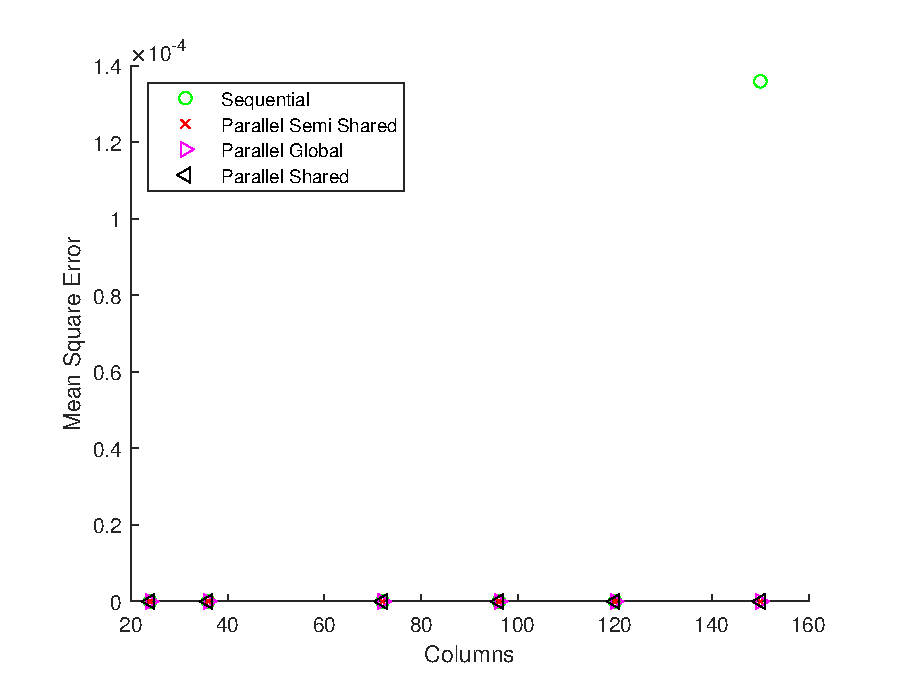
\includegraphics[width=.6\textwidth]{Grafici/Mean_Square_Error.eps} \label{fig:Mean_Square_Error}}
	\subfloat[][Dettaglio dell'errore quadratico medio]
	{\includegraphics[width=.6\textwidth]{Grafici/Mean_Square_Error_Zoom.eps} \label{fig:Mean_Square_Error_Zoom}} \\
	\caption{Confronto dell'errore quadratico medio}
\end{figure}
I grafici che seguono sono stati ottenuti usando la funzione \textit{cudaEventRecord} che registra un evento. Questa funzione permette di gestire due \textit{event}, chiamati \textit{start} e \textit{stop}, e di misurare il tempo intercorso tra i due. \textit{Start} viene registrato prima del ciclo \textit{while} presentato nel codice~\ref{code:sequential_loop}, mentre \textit{stop} quando si esce da questo loop. Dato che nel ciclo si esegue la One Sided Jacobi rotation si misura il tempo trascorso tra l'entrata e l'uscita del ciclo.

Le figure~\ref{fig:ColumnsTime} e~\ref{fig:ColumnsTime_Zoom} mostrano come cambia il tempo di esecuzione dell'algoritmo One-Sided Jacobi al variare della grandezza della matrice, in particolare del numero di colonne in quanto tutte le matrici di prova hanno lo stesso aspect ratio. L'algoritmo più veloce rimane quello che viene eseguito sull'host, mentre tra gli algoritmi testati sul device il migliore in termini di tempo è quello parallelo che usa la memoria shared. Questo è inoltre confermato dal fatto che questa è la memoria più veloce e può arrivare ad essere fino a 100 volte più veloce della memoria global. \cite{Cheng:ProfessionalCudaProgramming} \cite{Sanders:CudaByExample}
\begin{figure}[H]
	\centering
	\subfloat[][Relazione tra il numero di colonne\\ e il tempo di esecuzione]
	{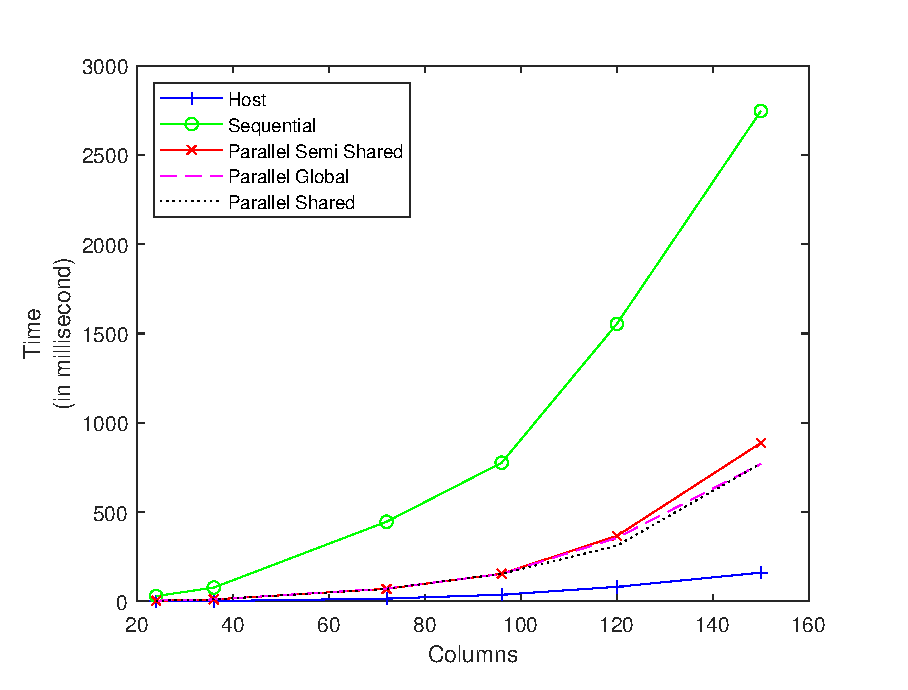
\includegraphics[width=.6\textwidth]{Grafici/ColumnsTime.eps} 
	\label{fig:ColumnsTime}}
	\subfloat[][Dettaglio Columns vs. Time]
	{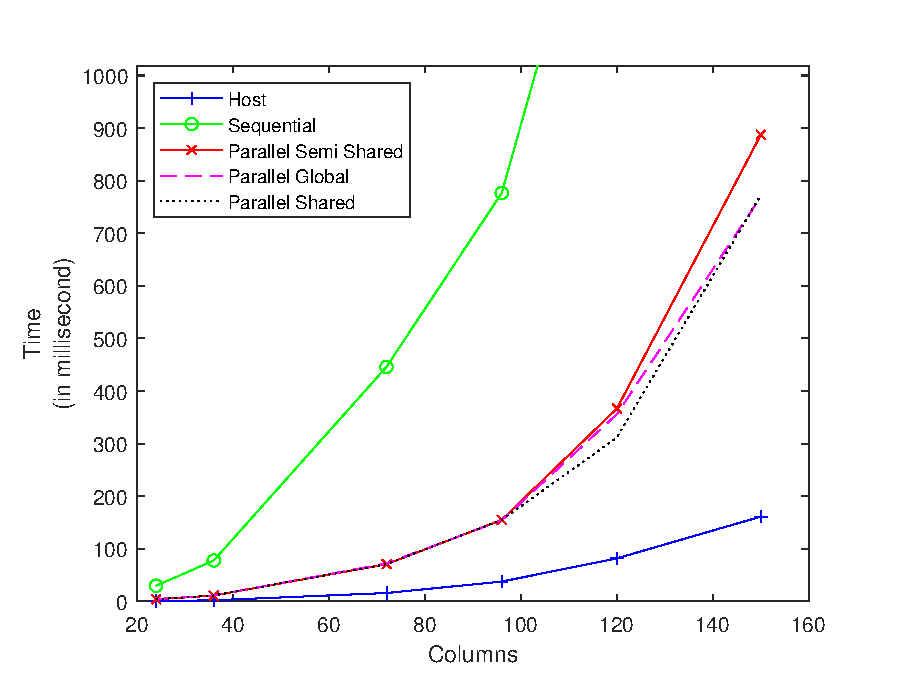
\includegraphics[width=.6\textwidth]{Grafici/ColumnsTime_Zoom.eps} \label{fig:ColumnsTime_Zoom}} \\
	\caption{Confronto Columns vs. Time}
\end{figure}
I grafici che seguono sono stati ottenuti usando lo strumento \textit{nvprof} che consente di raccogliere e visualizzare i dati di profiling dalla riga di comando. \textit{nvprof} consente la raccolta di una sequenza temporale di attività correlate a CUDA su CPU e GPU, tra cui l'esecuzione del kernel, trasferimenti di memoria e chiamate ad API CUDA ed eventi. Le opzioni di profiling vengono fornite a nvprof tramite le opzioni della riga di comando. Nei grafici di sinistra si possono notare le chiamate alle API CUDA, mentre in quelli di destra le prestazioni dei kernel. 

Sull'asse delle ordinate, la misura presa in considerazione è la percentuale di tempo sul totale del programma eseguito sul device. Sull'asse delle ascisse viene riportata la grandezza della matrice, in relazione al numero delle colonne. I grafici presentati sono divisi per tipo di algoritmo preso in considerazione.

Nei grafici~\ref{fig:API_Profiling_Sequential} e~\ref{fig:Kernel_Profiling_Sequential} vengono mostrate le prestazioni dell'algoritmo sequenziale. Nella figura~\ref{fig:API_Profiling_Sequential} si nota che per la matrice con 24 colonne le funzioni che occupano più tempo in percentuale sono \textit{cudaEventCreate} ($49\%$), \textit{cudaDeviceReset} ($23\%$), \textit{cudaLaunch} ($11\%$) e \textit{cudaMemcpy} ($11\%$), mentre per la matrice con 150 colonne sono \textit{cudaLaunch} ($82\%$) e \textit{cudaMemcpy} ($9\%$). La funzione \textit{cudaDeviceReset} distrugge tutte le allocazioni fatte e ripristina lo stato sul device, \textit{cudaLaunch} lancia una funzione del dispositivo. L'aumento della percentuale di tempo relativa a \textit{cudaLaunch} con l'aumentare della dimensione della matrice è conseguenza del fatto che il kernel \textit{rotate} viene richiamato $n(n-1)/2$ volte, dove $n$ è il numero di colonne, come spiegato nel capitolo~\ref{sec:Sequential} e come si può vedere nel codice~\ref{code:sequential_loop}. Il numero di volte con cui viene chiamata la funzione sul device ha andamento quadratico con l'aumentare delle colonne.

Il kernel che impiega più tempo, come si può vedere nella figura~\ref{fig:Kernel_Profiling_Sequential}, è \textit{rotate} per una percentuale di tempo maggiore del $99\%$.
\begin{figure}[H]
	\centering
	\subfloat[][Profiling delle API CUDA \\dell'algoritmo sequenziale]
	{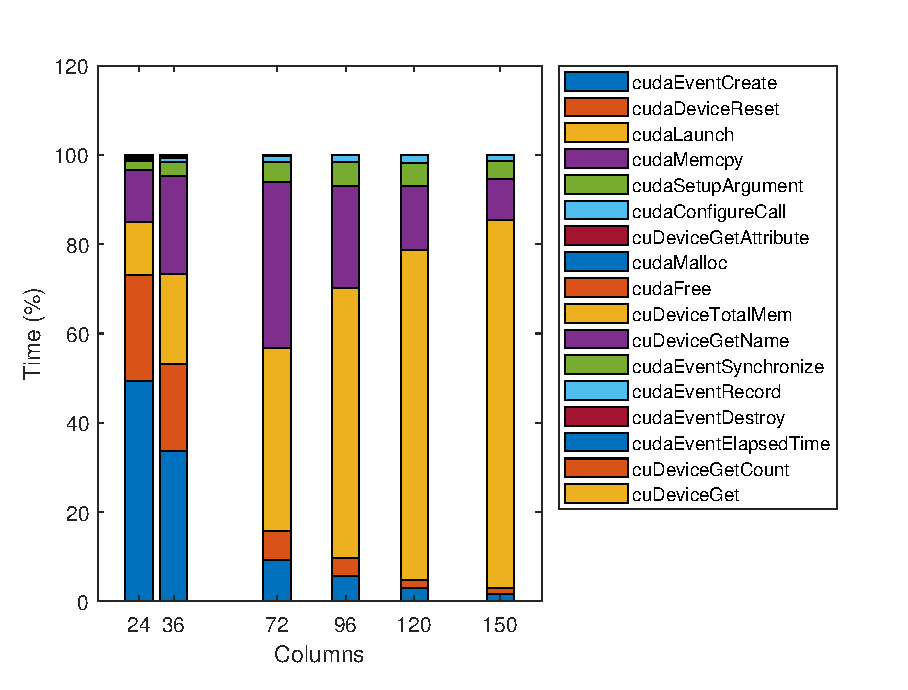
\includegraphics[width=.6\textwidth]{Grafici/API_Profiling_Sequential.eps} \label{fig:API_Profiling_Sequential}}
	\subfloat[][Profiling dei kernel \\dell'algoritmo sequenziale]
	{\includegraphics[width=.6\textwidth]{Grafici/Kernel_Profiling_Sequential.eps} \label{fig:Kernel_Profiling_Sequential}} \\
	\caption{Prestazioni algoritmo sequenziale}
\end{figure}

Nei grafici~\ref{fig:API_Profiling_Parallel_Global} e~\ref{fig:Kernel_Profiling_Parallel_Global} vengono mostrate le prestazioni dell'algoritmo parallel con la matrice \textit{B} salvata nella memoria globale. Come mostrato in figura~\ref{fig:API_Profiling_Parallel_Global}, le funzioni che richiedono più tempo per la matrice più piccola sono \textit{cudaEventCreate} ($58\%$), \textit{cudaDeviceReset} ($35\%$), \textit{cudaMemcpy} ($2\%$) e \textit{cudaLaunch} ($2\%$). Per la matrice più grande sono invece \textit{cudaMemcpy} ($88\%$), \textit{cudaEventCreate} ($5\%$), \textit{cudaDeviceReset} ($3\%$) e \textit{cudaLaunch} ($2\%$). Con l'aumentare della dimensione della matrice la funzione \textit{cudaMemcpy} ($88\%$) predomina dal punto di vista temporale perché occorre fare più copie dalla memoria dell'host a quella del device, e viceversa, della variabile \textit{host\_exit\_flag} come mostrato nel codice~\ref{code:parallel_loop}. 

Il kernel che impiega più tempo in percentuale è \textit{round} con l'$85\%$ per la matrice più piccola e il $96\%$ per quella più grande, mentre \textit{scheduling} impiega rispettivamente il $13\%$ e il $3\%$.

\begin{figure}[H]
	\centering
	\subfloat[][Profiling delle API CUDA \\dell'algoritmo parallelo global]
	{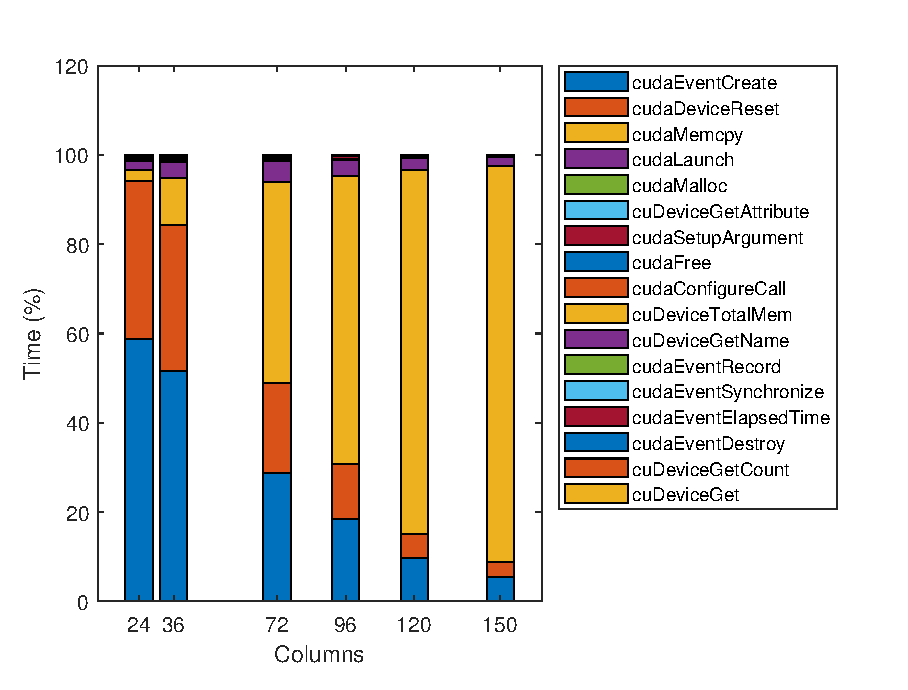
\includegraphics[width=.6\textwidth]{Grafici/API_Profiling_Parallel_Global.eps} \label{fig:API_Profiling_Parallel_Global}}
	\subfloat[][Profiling dei kernel \\dell'algoritmo parallelo global]
	{\includegraphics[width=.6\textwidth]{Grafici/Kernel_Profiling_Parallel_Global.eps} \label{fig:Kernel_Profiling_Parallel_Global}} \\
	\caption{Prestazioni dell'algoritmo parallelo global}
\end{figure}

Nei grafici~\ref{fig:API_Profiling_Parallel_Semi_Shared} e~\ref{fig:Kernel_Profiling_Parallel_Semi_Shared} vengono mostrate le prestazioni dell'algoritmo parallel con la matrice \textit{B} salvata nella memoria globale e con l'uso delle variabili all'interno del kernel salvate nella shared.

Le funzioni che impiegano più tempo per la matrice più piccola sono \textit{cudaEventCreate} ($56\%$), \textit{cudaDeviceReset} ($38\%$), \textit{cudaMemcpy} ($2\%$) e \textit{cudaLaunch} ($2\%$). Per la matrice più grande sono invece \textit{cudaMemcpy} ($89\%$), \textit{cudaEventCreate} ($4\%$), \textit{cudaDeviceReset} ($3\%$) e \textit{cudaLaunch} ($2\%$). 

Il kernel che impiega più tempo in percentuale è \textit{round} con l'$85\%$ per la matrice più piccola e il $96\%$ per quella più grande, mentre \textit{scheduling} impiega rispettivamente il $13\%$ e il $3\%$.

I risultati sono simili a quelli precedentemente descritti: la variazione più importante è nel tempo di esecuzione, mostrata nel grafico~\ref{fig:ColumnsTime_Zoom}, e non nella percentuale di tempo impiegata.

\begin{figure}[H]
	\centering
	\subfloat[][Profiling delle API CUDA \\dell'algoritmo parallelo semi-shared]
	{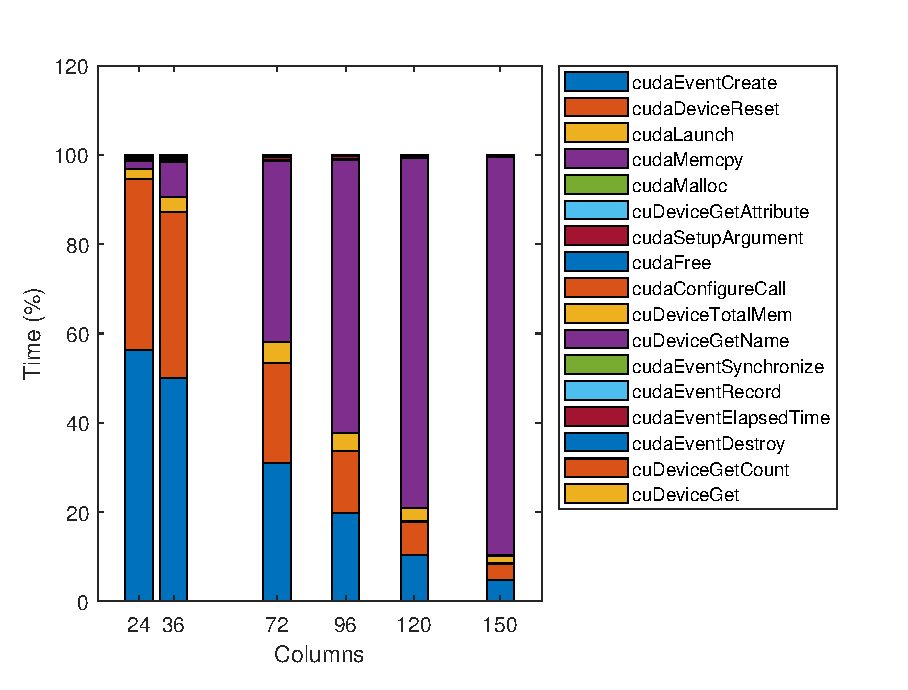
\includegraphics[width=.6\textwidth]{Grafici/API_Profiling_Parallel_Semi_Shared.eps} \label{fig:API_Profiling_Parallel_Semi_Shared}}
	\subfloat[][Profiling dei kernel \\dell'algoritmo parallelo semi-shared]
	{\includegraphics[width=.6\textwidth]{Grafici/Kernel_Profiling_Parallel_Semi_Shared.eps} \label{fig:Kernel_Profiling_Parallel_Semi_Shared}} \\
	\caption{Prestazioni dell'algoritmo parallelo semi-shared}
\end{figure}

Nei grafici~\ref{fig:API_Profiling_Parallel_Shared} e~\ref{fig:Kernel_Profiling_Parallel_Shared} vengono mostrate le prestazioni dell'algoritmo parallel con la matrice \textit{B} e le variabili usate nel kernel salvate nella shared memory.

Anche in questo caso i risultati sono simili a quelli precedentemente illustrati. L'uso della memoria shared per allocare il vettore diminuisce il tempo per completare il kernel \textit{round}, ma non la percentuale di tempo richiesta dalle singole funzioni.

\begin{figure}[H]
	\centering
	\subfloat[][Profiling delle API CUDA \\dell'algoritmo parallelo shared]
	{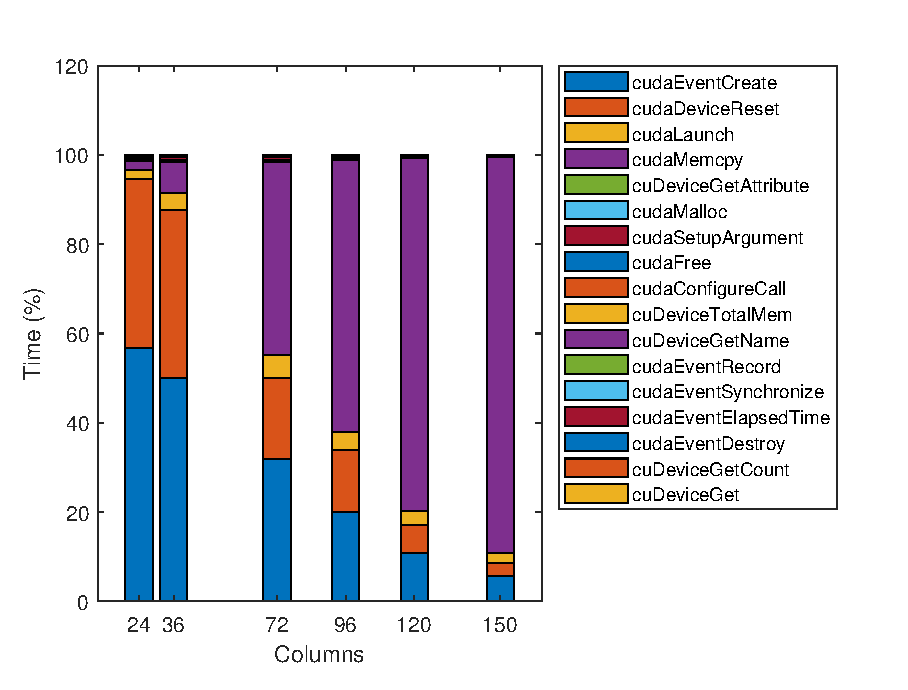
\includegraphics[width=.6\textwidth]{Grafici/API_Profiling_Parallel_Shared.eps} \label{fig:API_Profiling_Parallel_Shared}}
	\subfloat[][Profiling dei kernel \\dell'algoritmo parallelo shared]
	{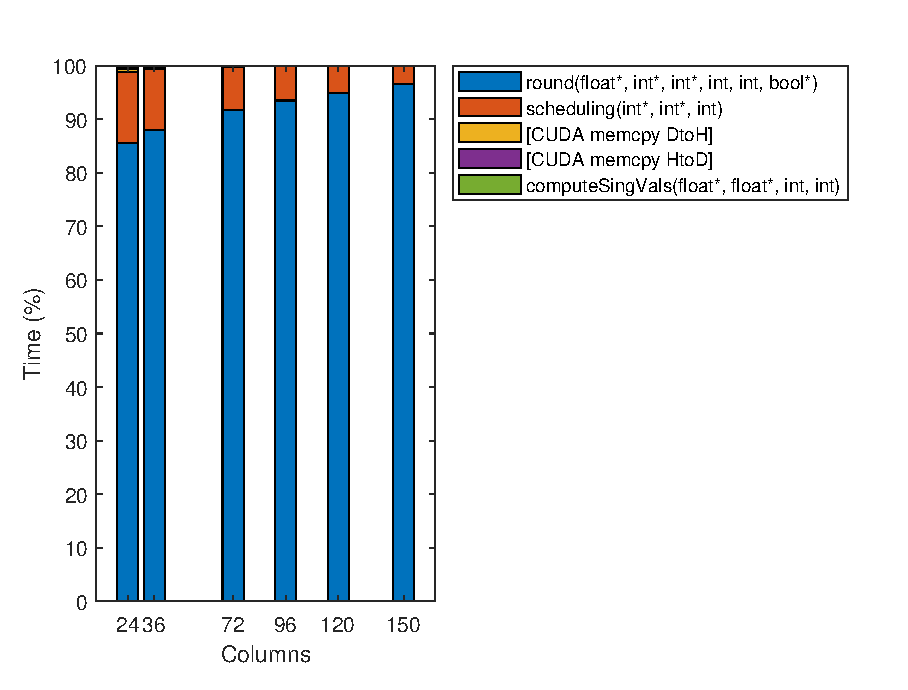
\includegraphics[width=.6\textwidth]{Grafici/Kernel_Profiling_Parallel_Shared.eps} \label{fig:Kernel_Profiling_Parallel_Shared}} \\
	\caption{Prestazioni dell'algoritmo parallelo semi-shared}
\end{figure}
